
\documentclass[12pt]{scrartcl} 


%----------------------------------------------------------------------------------------
%	PACKAGES AND OTHER DOCUMENT CONFIGURATIONS
%----------------------------------------------------------------------------------------

\usepackage{amsmath, amsfonts, amsthm} % Math packages

\usepackage{listings} % Code listings, with syntax highlighting

\usepackage[german]{babel} % English language hyphenation

\usepackage{graphicx} % Required for inserting images
\graphicspath{{Figures/}{./}} % Specifies where to look for included images (trailing slash required)

\usepackage{booktabs} % Required for better horizontal rules in tables

\numberwithin{equation}{section} % Number equations within sections (i.e. 1.1, 1.2, 2.1, 2.2 instead of 1, 2, 3, 4)
\numberwithin{figure}{section} % Number figures within sections (i.e. 1.1, 1.2, 2.1, 2.2 instead of 1, 2, 3, 4)
\numberwithin{table}{section} % Number tables within sections (i.e. 1.1, 1.2, 2.1, 2.2 instead of 1, 2, 3, 4)

\setlength\parindent{0pt} % Removes all indentation from paragraphs

\usepackage{enumitem} % Required for list customisation
\setlist{noitemsep} % No spacing between list items

%----------------------------------------------------------------------------------------
%	DOCUMENT MARGINS
%----------------------------------------------------------------------------------------

\usepackage{geometry} % Required for adjusting page dimensions and margins

\geometry{
	paper=a4paper, % Paper size, change to letterpaper for US letter size
	top=2.5cm, % Top margin
	bottom=3cm, % Bottom margin
	left=3cm, % Left margin
	right=3cm, % Right margin
	headheight=0.75cm, % Header height
	footskip=1.5cm, % Space from the bottom margin to the baseline of the footer
	headsep=0.75cm, % Space from the top margin to the baseline of the header
	%showframe, % Uncomment to show how the type block is set on the page
}

\usepackage[utf8]{inputenc} % Required for inputting international characters
\usepackage[T1]{fontenc} % Use 8-bit encoding
\usepackage{fourier} % Use the Adobe Utopia font for the document
\usepackage{sectsty} % Allows customising section commands

\sectionfont{\vspace{6pt}\centering\normalfont\scshape} % \section{} styling
\subsectionfont{\normalfont\bfseries} % \subsection{} styling
\subsubsectionfont{\normalfont\itshape} % \subsubsection{} styling
\paragraphfont{\normalfont\scshape} % \paragraph{} styling

%----------------------------------------------------------------------------------------
%	HEADERS AND FOOTERS
%----------------------------------------------------------------------------------------

\usepackage{scrlayer-scrpage} % Required for customising headers and footers

\ohead*{} % Right header
\ihead*{} % Left header
\chead*{} % Centre header

\ofoot*{\scriptsize Callum Stringer, Janik Spies und Fabrizio Franco} % Right footer
\ifoot*{\scriptsize Neue Wege - Bier brauen} % Left footer
\cfoot*{\pagemark} % Centre footer
\usepackage{pgf-pie}
\usepackage{pgfplots}

\linespread{1.241}

\usepackage{attachfile}

\usepackage{tablefootnote}

\usepackage{caption}
\newcommand{\source}[1]{\caption*{Quelle: {#1}} }


\usepackage[
backend=biber,
style=alphabetic,
sorting=ynt
]{biblatex}
\addbibresource{sample.bib}


\title{	
	\normalfont\small
	\textsc{Gibmit - VA - IBE17B}\\ 
	{Lehrperson - Herr Martin Meneghin}
	\vspace{25pt} 
	\rule{\linewidth}{0.5pt}\\
	\vspace{16pt} 
	{\huge Neue Wege - Bier brauen}\\ 
	\vspace{10pt} 
	\rule{\linewidth}{2pt}\\ 
	\author{\large Callum Stringer, Janik Spies und Fabrizio Franco} 
	\vspace{12pt} 
	\date{\small\today} 
}


\begin{document}

\maketitle
\thispagestyle{empty}
\newpage
\tableofcontents

\newpage
\section{Vorwort}
\subsection{Themenbegründung}
Die Entscheidung für das Brauen kam nicht sofort. Andere Ideen
 wie ein intelligenter Spiegel für das Badezimmer oder generell 
 ein Smarthome kamen uns in den Sinn. Wir hielten dies jedoch nicht
  für interessant genug. Als Gruppe beschlossen wir, ein Thema zu behandeln, das nicht direkt mit IT zu tun hat. Wir haben versucht, 
   ein Thema zu finden, das uns Spass macht, das neu und interessant ist und einen sozialen Aspekt hat.
Wir waren uns über das Brauen einig,
 da es etwas Neues ist. Etwas, das nicht jeder macht, 
 und das einen sozialen Aspekt hat, wenn man Brauer trifft und unser Bier mit Freunden und Familie testet.
 \subsection{Persönlicher Bezug - Janik Spies}
 Ich hatte keine wirkliche Idee für das Thema der VA. Callum ist dann mit der Idee gekommen die VA über die Bierbrauerei zu machen. Das hat mich angesprochen, da ich dieses Thema schon einmal privat angeschaut habe und auch schon einige Informationen über das Thema gesammelt habe. Ursprünglich bin ich auf das Thema Bierbrauerei gekommen, da ich öfters im Ausgang war und dort schon verschiedenste Biersorten versucht habe. Dabei hat mich aber keine richtig überzeugt. Deswegen habe ich auch schon dann überlegt, ob es sich nicht lohnen würde ein eigenes Bier zu Brauen. Schnell kam auch die Idee damit Geld zu verdienen. Im Idealfall würden wir beim Verkauf von Bier unseren Eigenkonsum decken und somit gratis unser Bier geniessen können. Auch das Bierbrauen in Grossbetrieben hat mich brennend interessiert, 
 da das zwei Leidenschaften von mir, Bier und Unternehmertum, zusammen verbindet.
\subsection{Persönlicher Bezug - Callum Stringer}
Mein persönlicher Bezug zur Brauerei war mir ungemein wichtig. Ich habe vorher zu Hause ein wenig gebraut. 
Ich war sehr begeistert, meine Vorkenntnisse in einem Schulprojekt einzusetzen. Obwohl ich schon Erfahrung habe, habe ich schon eine ganze Weile nichts gebraut.
 Ich hoffe, dass dieses Projekt mein Interesse und meine Motivation, noch etwas Bier zu brauen, wieder wecken wird.
 \subsection{Persönlicher Bezug - Fabrizio Franco}
 Meine Partner und ich haben uns zusammen für das Thema 'Bier brauen' entschieden. Ich war für dieses Thema, weil ich selber
  gerne Bier trinke aber nicht genau weiss, was in Bier enthalten ist oder wie überhaupt die Herstellung von Bier erfolgt. 
  Dazu kommt noch, dass mein Kollege Callum uns gut helfen kann, da er schon mal selber zuhause Bier gebraut hat und uns mit diesem 
  Experiment gut unterstützen kann. Es wundert mich zu wissen ob die Produktion von unterschiedlichen Sorten gleich abläuft oder 
  ob es bei bestimmten Sorten Abweichungen gibt. Mich interessiert auch zu wissen welche Unterschiede es bei der Herstellung von Bier
   zwischen Grossbrauereien wie Feldschlösschen und Kleinbrauereien gibt und wie die Preise für die verschiedenen Biersorten zustande 
   kommen. Hier in der Schweiz gibt es viele Kleinbrauereien und mich wundert es ob diese ein gewinnbringendes Geschäft oder eher eine
    Freizeit Beschäftigung sind. 
 Ich möchte mit diesem Projekt mein Wissen bezüglich Bier massiv erweitern da ich nur sehr weniger Erfahrung (abgesehen vom trinken) damit habe.
\subsection{\LaTeX\ }
Der Entschluss, \LaTeX\  als Werkzeug zur Dokumentenvorbereitung zu verwenden, wurde recht schnell gefasst. Wir haben \LaTeX\  bereits in
 der PVA verwendet. Es hat uns bei der Formatierung wirklich sehr geholfen und die Dinge einfach gehalten,
 so dass wir uns auf das Projekt konzentrieren konnten und uns keine Gedanken über das Herumfummeln mit Word machen mussten.
\\
Wir benutzten ein Git-Repository, um unsere Arbeit zu verfolgen, was es sehr einfach machte, als Team zusammenzuarbeiten. 
\subsection{Zusammenhang zwischen Klassen- und Gruppenthema}
Es war eine Herausforderung, eine Verbindung zwischen dem Bierbrauen und dem Thema 'Neue Wege' zu finden, aber man könnte es so betrachten, dass diese ganze Erfahrung, das Bierbrauen zu lernen, für uns ein neues Abenteuer und eine neue Erfahrung war. Man könnte also sagen, es war ein neuer Weg für uns als Gruppe.
\newpage
\subsection{Ziel und Zielbegründung}
\textbf{Finanziell lohnenswertes Bierbrauen}\\
Mit diesem Ziel wollten wir herausfinden, ob es sich finanziell lohnen würde sein eigenes Bier zu brauen. Dazu gehören die Herstellungskosten und die eventuellen Erträge durch den Bierverkauf. Unser Ziel dabei ist, die Kosten vom eigenen Bierkonsum so niedrig wie möglich zu halten.
\\\\\textbf{Kommerzielles Bierbrauen}\\
Mit diesem Ziel wollten wir herausfinden, wie das Bier in Grossbetrieben hergestellt wird und welche Unterschiede es zu den Heimbrauereien es gibt.
\\\\\textbf{Unterschied Alkoholfrei und Alkoholhaltig}\\
Bei dem Thema Bier hört man sehr oft das Thema alkoholfreies Bier. Uns hat interessiert, ob die Menschen einen Unterschied zwischen dem alkoholfreiem und dem alkoholhaltigen Bier erkennen. 
\\\\\textbf{Geschmacksergebnis bei der Eigenbrauerei}\\
Können wir ein geschmacklich vergleichbares Bier erstellen oder merken die Menschen den Unterschied zwischen dem selbst gebrauten Bier und dem gekauften Bier.
\\\\\textbf{Geschmackstest von Personen}\\
Können Personen in unserem Bekanntenkreis verschiedene Biersorten voneinander unterscheiden oder können sie das Bier nur am Etikett erkennen?

\newpage
\section{Einleitung}
\subsection{Einführung}
Brauen ist ein grosses Thema, wie man von dem Mindmap ablesen kann. 
Aber wir wollten uns auf einige wenige Themen konzentrieren.
Zunächst einmal haben wir uns für das Brauen selbst entschieden, 
wir wollten diese Erfahrung selbst durchgehen. Wir haben uns entschieden,
unser eigenes Bier mit Hilfe eines Bierkastens zu brauen. Dazu beschlossen wir auch,
eine Verkostungsveranstaltung durchzuführen, um zu sehen, ob unser Bier gut ist. 
Das zweite Thema, das wir uns anschauen wollten, ist, ob es sich lohnt, ein eigenes Bier zu brauen. Dazu gehörten die Finanzen des Bierbrauens und ob es billiger geht. Dazu gehört auch, ob das Bier gut genug schmeckt. Es könnte billig sein, aber es könnte sich nicht lohnen, wenn der Geschmack schlecht ist.
\\
Zu Referenzzwecken wird 'Vertiefungsarbeit' im gesamten Umfang dieses Dokuments als VA gekürzt
\newpage
\subsection{Mindmap}
Das Mindmap ist in den Beilagen ersichtlich, wir setzten uns hin und schrieben jede Idee auf, die uns in dieser Zeit in den Sinn kam. Danach nutzten wir diese als Planungshilfe und entschieden, welche Informationen und Themen wir untersuchen wollen.
Die Hauptthemen, für die wir uns entschieden haben, sind die folgenden:
\begin{itemize}
   \item Umgebung - Besuch der Brauereien, Interviews/Besuch in der Brauereien
   \item Biersorten - Beim Heimbrauen entschieden wir uns für spezifische Biersorten
   \item Herstellung
   \item Finanziell
   \item Design
\end{itemize}
Die folgenden Ideen wurden aufgrund der zeitlichen Beschränkungen dieses Projekts nicht geprüft:
\begin{itemize}
   \item Wirtschaft sowie Kultur
   \item Alkohol
   \item Umfrage
   \item Geschichte
\end{itemize}






\section{Hauptteil}
\section{Bierbrau Vorgang}
\subsection{Bierarten und Brauarten}
Es gibt viele Möglichkeiten, Bier und noch mehr Biersorten zu brauen.
Bier zu brauen gibt es schon so lange, wie es Menschen gibt. Es gibt sogar Aufzeichnungen über alte Eygpten und Mesopotamien \footnote{
	Mesopotamien oder Zweistromland bezeichnet die Kulturlandschaft in Vorderasien, die durch die großen Flusssysteme des Euphrat und Tigris geprägt wird.
}.\\
Jedes Getreide, das bestimmte Zucker enthält, könnte fermentieren. Da es wilde Hefen in der Luft gibt.
Das bedeutet, dass selbst in der Zeit der Stämme, als sie mit der Landwirtschaft begannen, eine Art Bier hergestellt worden sein könnte.\\
Das meiste Bier wird aus einer Art Stärkequelle hergestellt, die fermentiert werden kann, Brauereihefe zur Herstellung und Einleitung der
Gärung und Aromatisierung wie Hopfen, um die Süße des Zuckers auszugleichen

\subsection{Bestellung}
Zur Vorbereitung des Bierbrauens benötigten wir Materialien.
Wir entschieden uns für die Verwendung von "Bier-Kits". Aus Zeitgründen war es nicht möglich,
das Bier auf traditionelle Weise zu brauen, da dies zu lange dauern würde.
Wir bestellten zwei verschiedene Kits, von denen das eine ein Cherry Ale und das andere ein belgisches Saisonbier war.
Wir haben uns für diese beiden Biere entschieden, zum einen, weil wir einen Grundtyp von Bier brauen wollten, zum anderen, weil wir etwas experimentelleres brauen wollten.  Das experimentelle ist das Cherry Ale. Wir hatten so etwas in der Schweiz noch nie so leicht erhältlich gesehen und wollten es unbedingt ausprobieren.
Der zweite Grund war die Verfügbarkeit. Wir hatten uns schon früher für Tyuoes entschieden, und sie waren nicht schnell verfügbar. Und wegen des Zeitdrucks bei diesem Projekt mussten wir das nehmen, was von Anfang an verfügbar war.

Wir hatten bereits Ausrüstung, um das Bier selbst zu brauen, wie Callum Stringer dies schon einmal getan hatte.
Unsere definitive Reihenfolge war wie folgt.

\textbf{Schon vorhandene Artikel}
\begin{itemize}
	\item Starter-Paket de Luxe für Bierkits - Preis CHF 79.00
\end{itemize}
\textbf{Neu bestellte Artikel}
\begin{itemize}
	\item Bügelflasche braun kompl. 0,5 L - Preis CHF 126.00
	\item Brewferm Bierkit Cherry Ale - Preis CHF 29.00
\end{itemize}

Als wir die Bestellung erhielten, stellten wir fest, dass uns ein Fehler unterlaufen war, und bestellten 60 Bierflaschen,
 wobei wir davon ausgingen, dass jeder Satz 15 Liter ergeben würde. Dies bedeutete, dass wir genau genug Flaschen für das gesamte Bier haben würden.
 Je nach Art des Kits war die gebraute Biermenge jedoch unterschiedlich. Wir hatten also viel zu viele Flaschen.

 \begin{figure}[!h]
	\centering
	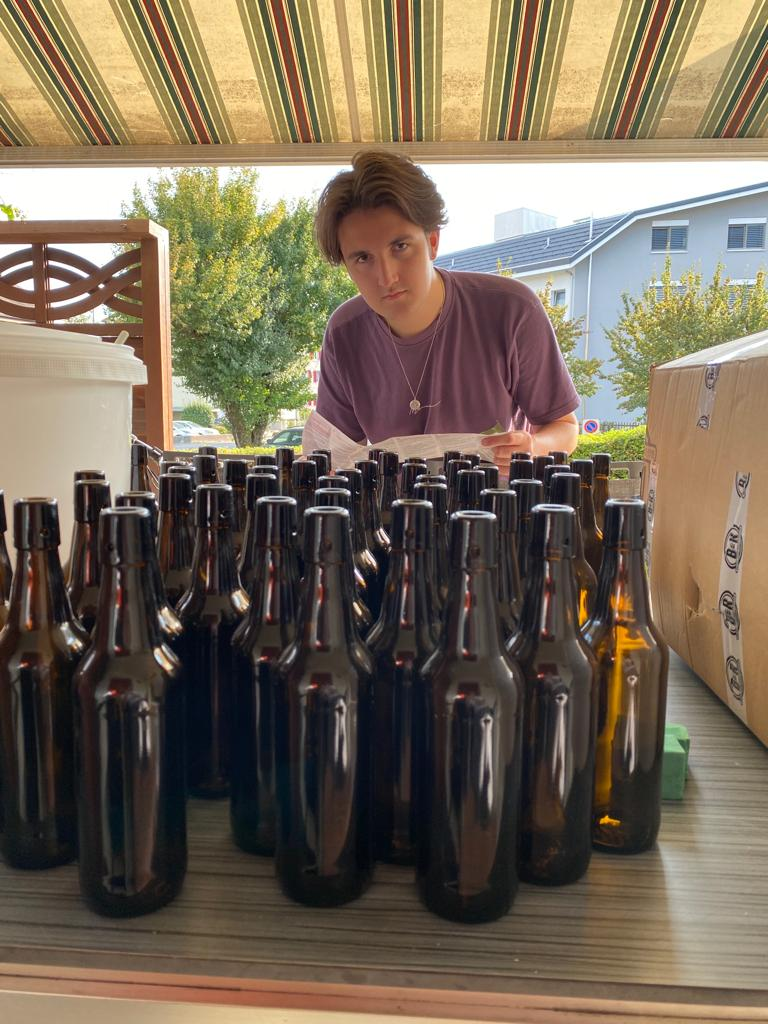
\includegraphics[width=0.5\columnwidth]{callum.png}
	\caption{Kontrolle der Bestelle Artikeln}
\end{figure}

\subsection{Vorbereiten}
\subsubsection{Disinfektion}
Zunächst einmal mussten wir alles vollständig reinigen.
Dazu bereiteten wir eine Desinfektionslösung mit den im Bierkit enthaltenen Mischgranulaten vor.
Dies war wichtig, da wir nicht wollen, dass etwas Unbekanntes im Bier ist, wenn es gärt.
Danach konnten wir mit dem eigentlichen Brauen des Bieres fortfahren. \\

Die Desinfektion hat einige Zeit in Anspruch genommen. Wir haben das Bier im Haus von Fabrizio Francos Familie gebraut.
Und Platz zu finden, um die großen Eimer durchgehend zu reinigen,
war eine echte Herausforderung. Am Ende haben wir viele der Reinigungsarbeiten in der Badewanne durchgeführt.
Hier gab es auch einige andere Herausforderungen. Die Desinfektionslösung war nicht die neutralste Flüssigkeit.
Callum Stringers dazu zu bringen, die Hände jucken und zornig zu machen. Danach entschieden wir uns für die Verwendung von Reinigungshandschuhen.
Der Prozess verlief danach sehr viel reibungsloser


\begin{figure}[!h]
	\centering
	
\includegraphics[width=0.5\columnwidth]{fabi.jpg}
	\caption{Disinfektion der Fass}
\end{figure}


\subsubsection{Bierkit vorbereitung}
Zuerst mussten wir die Bausätze öffnen. Nach dem Öffnen mussten wir sie aufwärmen. Dazu legten wir
sie etwa 15 Minuten lang in eine mit Wasser gefüllte Pfanne bei schwacher Hitze. Sobald es warm war,
wurde es in die großen Braubehälter gegossen. Danach fügten wir das Wasser hinzu. Je nach Art des Bierkits
geschah dies in verschiedenen Schritten. Zuerst warmes Wasser, dann lauwarmes Wasser auf die Gesamtmenge.
Einige dieser Wasserchargen waren Zuckerlösungen. Da die Hefe Zucker zum Leben und Wachsen braucht.
Danach hatten wir zwei große Fässer des jungen Bieres.
Dieses musste vor der Abfüllung gelagert werden, wir legten es in den Kasten und ließen es dort für 10 Tage stehen.
Wenn man das Bier sotriert, muss man darauf achten, wo und unter welchen Bedingungen es gelagert wird.
Damit die Hefe einwirken kann, muss die Hefe in der ersten Brauphase relitavly warm sein, jedoch nicht zu warm und ungünstig an einem dunklen Ort. 
Denn direkte Sonneneinstrahlung kann die Hefe leicht abkühlen, und ohne Hefe gibt es kein Bier!
Außerdem muss man darauf achten, dass die Flasche bzw. das Fass gut verschlossen ist. Wir haben wegen des billigen Materials,
aus dem das Fass hergestellt ist, bemerkt, dass die Möglichkeit von Undichtigkeiten besteht. Wie Sie auf dem folgenden Bild sehen können,
haben wir einige Papierzwillinge zurückgelassen, falls während der Lagerung Bier ausgelaufen sein sollte. \\



\begin{figure}[!h]
	\centering
	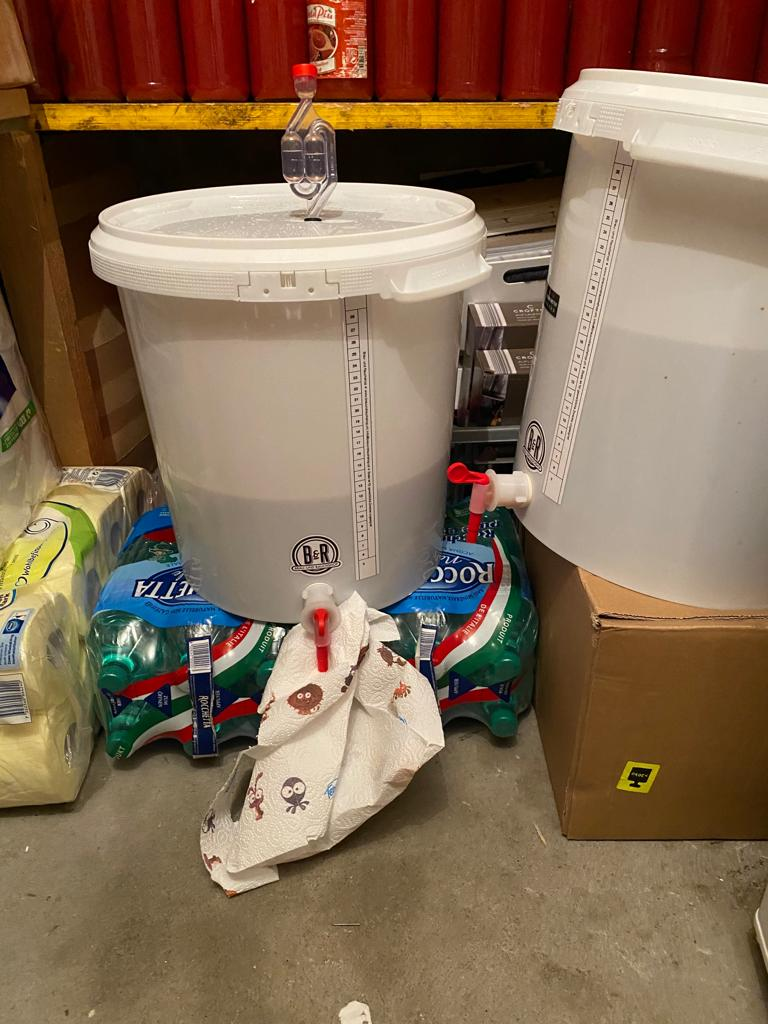
\includegraphics[width=0.5\columnwidth]{barrels.jpg}
	\caption{Lagerung der Bier}
\end{figure}
\newpage

\subsubsection{Bier in Flaschen abfüllen}
Bevor wir mit dem Abfüllen des Biers in die Glasflaschen angefangen haben, mussten wir alle neuen und alten Flaschen waschen. Wir haben 6 Liter Wasser und 5 Gram Waschmittel in einem Korb eingefüllt und gemischt. Nach 5 Minuten fingen wir an die Flaschen in dem Korb rein zu tun und liessen sie für eine Minute im Wasser stehen und spülten sie danach ab um jeden Schmutz, welcher sich in den Flaschen gesammelt hat zu entfernen. Dies dauerte länger als erwartet, da wir alle vorhandenen Flaschen gewaschen haben und diese um die 90-100 Flaschen waren. Nach dem abwaschen gaben wir jeder Flasche einen auf- und schliessbaren Deckel. Die Flaschen sahen alle gleich aus und damit wir kein durcheinander haben, fingen wir mit der Produktion von dem Cherry Ale an. Wir hatten nur 12 Liter von diesem Ale und jede Flasche hatte eine Kapazität von 0,5 Liter d.h. für 12 Liter waren es 24 Flaschen. Nachdem wir 1,5 Stunden gebraucht haben um alles zu reinigen und trocknen, haben wir die ersten 24 Flaschen auf dem Tisch gestellt. Dann fing der Spass erst an. Am Braugefäss war ein Schlauch zum Abfüllen angehängt und dieser war so präpariert, dass wenn man den Anfang des Schlauchs gegen etwas drückt fing das Bier an zu strömen und wenn kein Druck mehr stattfand hörte es auf. Durch ein Ventil welches am Braugefäss angebaut war, konnten wir den Durchfluss des Biers starten und stoppen.
Wir öffneten das Ventil, steckten den Schlauch in die Flasche und drückten es gegen den Flaschenboden bis es bis zum Flaschenhals voll mit Bier war, machten aber die Flaschen noch nicht mit dem Deckel zu weil noch eine Zutat fehlte. Nachdem wir alle 24 Cherry Ale Flaschen abgefüllt hatten verstauten wir diese für den Moment in einer Kiste und stellten die neuen Flaschen für «das andere Ale wo mir jetzt grad nid ihfallt» auf dem Tisch und führten den gleichen Vorgang erneut aus. Diese Flaschen stellten wir in eine separate Kiste. Jetzt fehlte nur noch das Einfügen des Zuckers. Dieser Vorgang war nicht so leicht und ein bisschen hektisch. Wir stellten auf den vorbereiteten Flaschen einen Trichter, zum einfüllen von einem Esslöffel Zucker. Dies musste aber eingefüllt und die Flasche schnell verschlossen werden. Wir hatten einen Zeitraum von 3 Sekunden um beides zu machen und waren wir zu langsam, schäumte das Bier über und es gab eine riesige Sauerei. Dies machten wir für alle 90 Flaschen und zum Glück geschah dies nur einmal über den ganzen Vorgang. Danach verstauten wir die Flaschen wieder getrennt in die Kisten und liessen sie für mehrere Wochen stehen.


\section{Bier Labels}
\section{Finazialle Sicht}
\newpage
\section{Degustation}
\subsection{Planung}
\subsubsection{Ziel der Degustion}
\begin{itemize}
    \item Erkennen die Befragten den Unterschied zwischen alkoholfreiem und alkoholhaltigem Bier?
    \item Können wir als Anfänger ein vergleichbares Bier herstellen?
    \item Wie wird unser Bier bewertet?
\end{itemize}

\subsubsection{Durchführung}
Wir verwenden Plastikbecher und markieren diese mit folgendem Farbschema:
\begin{itemize}
    \item Blau: 	Selbstgebrautes Weizenbier
    \item Rot:		Selbstgebrautes Cherry Ale
    \item Gelb: 	Feldschlösschen Braufrisch 
    \item Grün:		Chouffe Cherry Ale 
    \item Schwarz:	Appenzeller Weizenbier (Alkoholfrei) 
\end{itemize}
\paragraph{}
Danach werden die Biersorten in die dafür vorgesehenen Plastikbecher abgefüllt. Es soll somit vermieden werden, dass die Teilnehmer wissen, um welches Bier es sich jeweils handelt.
Wir bitten die Teilnehmer dann jeweils eine Biersorte nach der anderen zu probieren und dabei das Auswertungsblatt, welches weiter unten zu finden ist, auszufüllen. Mit dieser Methode ist es uns möglich herauszufinden, ob die Testpersonen unser Bier mögen oder einen Unterschied von alkoholhaltigem und nicht alkoholhaltigem Bier herausschmecken können. Weiter werden wir bei der Wahl darauf achten, möglichst unterschiedliche Altersgruppen und Alkoholkonsumenten einzuladen, so dass wir gegebenenfalls einen Unterschied zwischen Altersgruppen und den verschieden starken Alkoholkonsumenten herausfinden können.
\\
\textbf{Design:}\\
Aktuell haben wir nur die «nackten» Bierflaschen. Da wir aber bei der Degustation und vor allem auch bei der Präsentation einen ästhetisch ansprechenden Auftritt liefern wollen, haben wir und dazu entschieden Labels für die Flaschen zu erstellen. Diese Aufgabe haben wir mit Photoshop und Etikettenpapier bewältigen. Wir haben mehrere Designs erstellt und uns für die zwei folgenden entschieden:

\begin{figure}[!h]
    \centering
    \begin{minipage}{.5\textwidth}
      \centering
      
\includegraphics[width=.7\linewidth]{Cherry.png}
      \captionof{figure}{Cherry Ale Design}
      \label{fig:test1}
    \end{minipage}%
    \begin{minipage}{.5\textwidth}
      \centering
      
\includegraphics[width=.7\linewidth]{Figures/Wheat.png}
      \captionof{figure}{Wheat Design}
      \label{fig:test2}
    \end{minipage}
\end{figure}

\textbf{Allgemein:}
Es war uns wichtig, dass das Design simpel und ansprechend aussieht. Dazu waren wir limitiert, da unser Etikettenpapier uns nicht viel Platz bat. Da wir das Bier nicht kommerziell nutzen, mussten wir auch keine Angaben über die Inhaltsstoffe andrucken, was uns natürlich viel Ärger erspart hat. Der Äussere Ring dient als Platzhalter für den Titel und den Alkoholgehalt. In der Mitte haben wir einen dunkleren Hintergrund und das Logo, welches mit einem leichten Schlagschatten heraussticht.
\\
\textbf{Cherry Ale:}
Die Kirsche vom Cherry Ale Logo wurde von dem Unternehmen «MX CHERRY»  inspiriert. Farblich haben wir uns für ein dunkles Weinrot entschieden, da wir fanden, dass das zu Kirschen passen würde. Der kapitalisierte und verzerrte Titel sorgt für Aufmerksamkeit und das Logo sticht von der Mitte hervor.
\\
\textbf{Weizen Bier:}
Beim Weizenbier wollten wir natürlich auch in dem gleichen Stil bleiben, jedoch sollte jedermann einen klaren Unterschied zwischen den Biersorten erkennen. Dies haben wir mehrheitlich durch die Farbe und dem Symbol erzeugt. Hier haben wir die Kapitalisierung des Titels weggelassen, um dem Symbol eine grössere Aufmerksamkeit zu widmen. 

\section{Lernziel}
\section{Schlussbetrachtung}
\subsection{Schlusswort}
\subsubsection{Inhaltliche Schlusswort}
Während dieses Projekts haben wir eine Menge über das Brauen gelernt. Wir haben den Prozess des Bierbrauens selbst durchlaufen. Wir fanden auch heraus, wie sehr das Brauen ein grosses Thema ist und wie tief man in die Tiefe gehen kann. Wir fanden es interessant, Bier aus einer kleinen Wanne in einem Haus zu brauen. Es war eine Erfahrung, die sehr interessant und voller lustiger Momente war. 

Unser Bier kam recht gut heraus.
 Als Gruppe haben wir beschlossen, dass uns das Bier schmeckt. 
 Was für uns aber auch wichtig war, war, wie andere Leute darüber dachten.
  Unsere Verkostungsveranstaltung verlief gut, und wir waren mit den Ergebnissen zufrieden.
   Wir hätten nie erwartet, dass es das am besten schmeckende Bier sein würde, aber dass die Leute 
   keine grossen Probleme damit hatten, war für uns grossartig.

\subsubsection{Zielkontrolle}
\textbf{Finanziell lohnenswertes Bierbrauen}\\
Wir konnten im Kapitel 4.1 genau sehen, dass es sich finanziell nicht lohnen würde sein eigenes Bier zu produzieren. Der Verkaufspreis müsste um weites höher sein als die der Marktgegner. Wir haben unser Ziel zwar erreicht, da wir vorerst nur herausfinden wollten, ob es sich lohnen würde. Aber wir konnten unser Unterziel, es finanziell Lohnenswert zu machen nicht erreichen.
\\
\textbf{Kommerzielles Bierbrauen}\\
Leider konnten wir dieses Ziel bislang nicht erreichen, da uns alle Brauereien abgesagt haben oder sich nicht mehr gemeldet haben. Trotzdem bleiben wir offen und schauen, dass wir das Ziel eventuell noch bis zur Präsentation der VA erreichen können.
Unterschied Alkoholfrei und Alkoholhaltig
Durch die Degustation konnten wir dieses Ziel sehr leicht erreichen. Dabei wurden die Testpersonen jeweils gefragt, ob sie denken, dass das getestete Bier alkoholfrei oder alkoholhaltig ist. Dabei wurde schnell klar, dass die Mehrheit einen klaren Unterschied erkennt.
\\\newpage
\textbf{Geschmacksergebnis bei der Eigenbrauerei}\\
Auch dieses Ziel wurde in der Degustation erreicht. Dabei wurden verschiedene Biersorten, unter anderem auch unser selbst gebrautes Bier, miteinander verglichen und bewertet. Unser Bier wurde dabei immer ein wenig schlechter bewertet als die gekauften Biersorten, jedoch konnte es trotzdem sehr gut mithalten.
\\
\textbf{Geschmackstest von Personen}\\
Dieses Ziel wurde ebenfalls bei der Degustation erreicht, indem wir die Befragten mit der Auswahl der Biersorte untersuchten. Dabei kam heraus, dass es einige gibt, für die es sehr schwer war das Weizen- und Hopfenbier zu unterscheiden. Somit kann man sagen, dass es in Abhängigkeit zu der Biersorte viele Leute gibt, die Biersorten nicht wirklich unterscheiden können.
\\

\subsubsection{Persönliche Reflexion - Fabrizio Franco}
Dieses Projekt war wahrscheinlich eins der besten und lustigsten, an denen ich mich je selber beteiligen durfte. Ich freue mich im Nachhinein sehr, diesen Auftrag, mit Callum und Janik ausgeführt zu haben. Wir hatten viel Spass bei der Zubereitung des Biers und beim Planen des ganzen Auftrags. Ich habe viele neue Kenntnisse im Zusammenhang mit der Herstellung von Bier und den verschiedenen Brauarten gemacht. Ich selber war noch nie in einer Brauerei und wusste vor diesem Projekt gar nicht aus was Bier besteht und wie dieses überhaupt zustande kommt. Durch diesem Auftrag habe ich eine Art des Bierbrauens kennengelernt und konnte mein Wissen erweitert und habe dazu gemerkt, dass es nicht so schnell geht, wie ich es mir erhofft hatte, das frisch gemachte Bier zu trinken. Es musste mehrere Wochen lang ruhen, damit das Bier gut ist und genossen werden kann. Probleme tauchten eigentlich keine auf. Das einzige was man als "kleines Problem" betrachten könne, ist dass das Bier beim Öffnen der Flasche überschäumt. Doch trotz dessen kann man es, nach einigen Minuten warten, genussvoll trinken und geniessen. Die Degustation mit meinen Freunden durchführen gedurft zu haben, war für mich eines der besten Erlebnissen dieser Vertiefungsarbeit und es hat mich glücklich gemacht, dass das Bier ihnen gefallen hat. Im Grossen und Ganzen hat mir diese Arbeit sehr viel Spass bereitet und ich denke
 wir haben ein tolles Projekt auf die Reihe bekommen und wir sind glücklich mit unserem Ergebnis und dem Bier.
\subsubsection{Persönliche Reflexion - Callum Stringer}
Ich habe diese Arbeit sehr genossen. Ich habe mich in der Vergangenheit immer für das Brauen interessiert. Es ist sehr befriedigend, draussen zu sitzen und sein selbstgebrautes Bier zu trinken, nachdem man einen Tag Arbeit und wochenlanges Warten hinter sich gebracht hat.
Ich genoss die Erfahrung, als ich es alleine machte, aber dieses Hobby mit einigen Freunden zu teilen, hat mir sehr viel Spass gemacht.
Ich scheine im Laufe des Prozesses eine Menge Dinge zu lernen. Viele kleine Tipps und Tricks, an die ich mich in Zukunft erinnern werde.
Zum Beispiel ist es wichtig, etwas Papier unter den Zapfhahn des Fasses zu legen, da ich früher klebriges Bier vom Boden reinigen musste,
nachdem ich es tagelang nicht kontrolliert hatte.
Eine andere Sache ist es, vorbereitet zu sein und alles bereit zu haben, wie eine Art Mise en Place. Das macht es später einfacher, da man
nicht alles suchen muss.
Ein weiterer Punkt ist, dass das Fass vor der Herstellung des Bieres leicht erscheinen mag, aber 20 Liter Bier sind ziemlich schwer,
und es in der Küche zuzubereiten und es dann vorsichtig nach unten tragen zu müssen, war nicht die einfachste Sache.

Abgesehen vom Bier lief das Projekt als Ganzes gut, wir hatten einige Probleme mit dem Zeitmanagement in der PVA, aber dieses Mal haben wir uns einen Moment Zeit genommen, um anzuhalten und den gesamten Prozess zu planen. Dafür schufen wir ein Trello-Board. Mit diesem kann man To-Dos hinzufügen und den Fortschritt bei bestimmten Aufgaben verfolgen. Es war sehr nützlich, einen Überblick darüber zu behalten, was getan werden musste.
\newpage
\subsubsection{Persönliche Reflexion - Janik Spies}
Mir hat die VA sehr gut gefallen. Wie auch schon oben erwähnt habe ich einen engen Bezug zum Thema Bier und wollte auch unbedingt wissen, ob sich das Bierbrauen finanziell lohnen würde. Es hat mich jedoch sehr enttäuscht, dass wir vor allem aufgrund vom Corona keinen Besuch in einer Brauerei machen konnten. Dort hätten wir noch sehr viele Informationen bekommen, vor allem was den Bereich Verkauf angehen würde. Aber abgesehen von dem, hatten wir sehr viel Spass bei der VA und vor allem beim Bierbrauen und Testen. Es gab viele spannende und lustige Momente, auf die ich bei der Präsentation noch genauer eingehen werde. Auch mit dem Erreichen unserer Ziele bin ich sehr zufrieden.



\nocite{*}
\printbibliography[title={Quellenverzeichnis}]
\addcontentsline{toc}{section}{Quellenverzeichnis}

\listoffigures

\renewcommand{\listfigurename}{Abbildungsverzeichnis}
\renewcommand{\listtablename}{Tabellenverzeichnis}
\addcontentsline{toc}{section}{Abbildungsverzeichnis}
\addcontentsline{toc}{section}{Tabellenverzeichnis}


\vspace*{4em}\noindent
\hfill%
\begin{tabular}[t]{c}
	\rule{10em}{0.4pt} \\ Callum Stringer
\end{tabular}%
\hfill%
\begin{tabular}[t]{c}
	\rule{10em}{0.4pt} \\ Datum
\end{tabular}%
\hfill\strut

\vspace*{4em}\noindent
\hfill%
\begin{tabular}[t]{c}
	\rule{10em}{0.4pt} \\ Fabrizio Franco
\end{tabular}%
\hfill%
\begin{tabular}[t]{c}
	\rule{10em}{0.4pt} \\ Datum
\end{tabular}%
\hfill\strut

\vspace*{4em}\noindent
\hfill%
\begin{tabular}[t]{c}
	\rule{10em}{0.4pt} \\ Janik Spies
\end{tabular}%
\hfill%
\begin{tabular}[t]{c}
	\rule{10em}{0.4pt} \\ Datum
\end{tabular}%
\hfill\strut

\end{document}
